\setcounter{chapter}{5}
\chapter{Shortest Path}%
\label{chap:06}

Examples where shortest path algorithms are used in computer vision
\begin{itemize}
\item Intelligent scissors (GIMP)/ Magnetic lasso (Photoshop)
\item Geodesic matting/ seeded segmentation
\item segmented least squares (estimate piecewise constant best
  approximation, but a cost is imposed on jumps in the resulting
  function)
\end{itemize}

Basic approach to tackle shortest path problems: \textbf{dynamic
  programming}. Generally problems where dynamic programming
techniques are applied are required to have the \emph{optimal
  subproblem} property, which means that the optimal solution to a
partial problem has to be part of the overall optimal solution.
\begin{example*}[Shortest path]
  Consider the following graph:
  \begin{figure}[h!]
    \centering
    \begin{tikzpicture}
      \node[shape=circle,draw,inner sep=2pt] (S) at (0,0) {$s$};
      \node[shape=circle,draw,inner sep=2pt] (K) at (3,1) {$k$};
      \node[shape=circle,draw,inner sep=2pt] (T) at (5,3) {$t$};

      \draw[-] (S) to (K); \draw[-, red] (S) to[bend right=5] (K);
      \draw[-] (K) to (T);
    \end{tikzpicture}
  \end{figure}
  
  We do not know if the shortest path from $s$ to $t$ will go through
  $k$; if it does go through $k$, however, the the shortest path
  $s \rightarrow k$ must be part of the globally optimal shortest path
  $s \rightarrow t$ (red path).
\end{example*}
It only makes sense to use dynamic programming if the solutions of the
subproblems can be re-used multiple times.

\setcounter{section}{1}
\section{Shortest path algorithms}%
\label{sec:shortpathalgo}

In the following, the length of a path is defined to be the sum of the
edge weights.

\todo{Dijkstra and Viterbi with example from lecture}

\section{Scanline optimization/ Stereo disperity estimation}
Setting: Two cameras, slighlty shifted or rotated and rectified, take
two pictures of the same scene. We want to estimate the ``depth'' of
the elements in the scene. As illustrated in the image below, the two
pictures are evaluated along a horizontal scanline (the example is
taken from \url{http://lunokhod.org/?p=1356}).

\begin{figure}[h!]
  \centering
  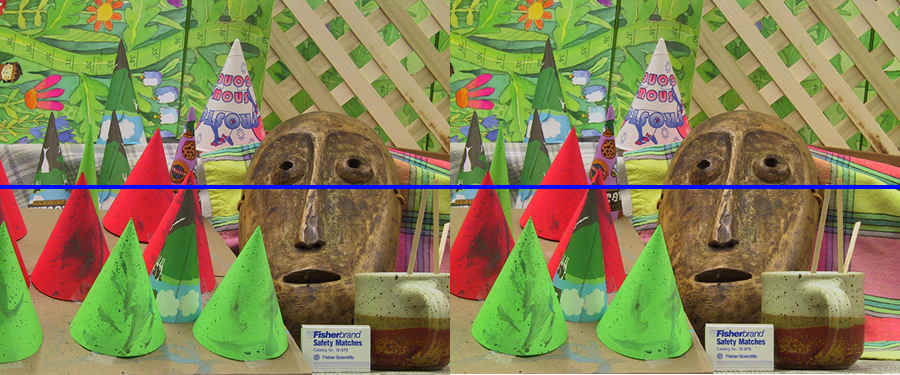
\includegraphics[width=0.9\textwidth]{Figures/input_imagery_and_scanline}
  \caption{Original rectified stereo images}
\end{figure}
For each pixel along that line, each possible disparity result is
evaluated. The cost of each pixel along a scanline can then be stacked
into a matrix; the cost for each pixel on the scanline in the example
image versus each possible disparity value is shown in the Figure
below. The solution for the disparity along this scanline is then the
path through this matrix (image) that has minimum costs (dark areas)
with some smoothness constraint imposed (\ie, the shortest path). The
process is repeated for every horizontal scanline; the resulting
disparity map is given in Figure~\ref{fig:disperity_map}. Since each
scanline is treated individually, the result might be not very smooth
in the y-direction and one can apply different smoothing techniques to
obtain a disparity map this is smooth in both the x- and y-direction.

\begin{figure}[h!]
  \centering
  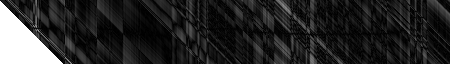
\includegraphics[width=0.9\textwidth]{Figures/scanline_costs}
  \caption{All possible disparities along one scanline}
\end{figure}     


\begin{figure}[htpb]
  \centering
  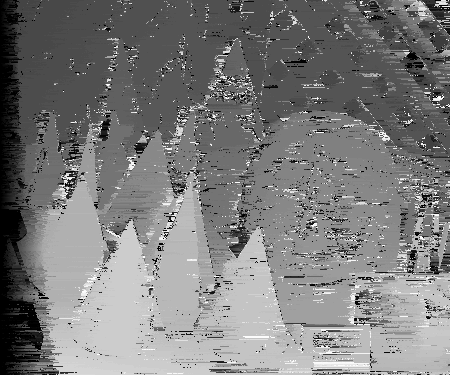
\includegraphics[width=0.7\textwidth]{Figures/cones_scanline_optimization_only}%
  \caption{Disparity map for the example above}%
  \label{fig:disperity_map}
\end{figure}

\section*{MAP -- maximum a posteriori estimation}
The problem above can be rewritten as: Find
\begin{align*}
  \min_{z_1, \dotsc, z_n}e(z) &= \min_{z_1, \dotsc, z_n} \sum_{i=1}^{n-1} \psi_{i,i+1}(z_i, z_{i+1}) \\
                              &= \min_{z_1, \dotsc, z_n} \psi_{n-1,n}(z_{n-1}, z_n) + \dotsm + \psi_{2,3}(z_{2}, z_3) + \psi_{0,1}(z_{0}, z_1) \\
                              &= \min_{z_n}\Bigg(
                                \min_{z_{n-1}}\psi_{n-1,n}(z_{n-1},z_n) + \dotsm + \min_{z_2}\Big(
                                \psi_{2,3}(z_2, z_3) + \underbrace{\min_{z_1}\psi_{1,2}(z_1, z_2)}_{
                                m_{1\rightarrow 2}(z_2)
                                }
                                \Big) \dotsm
                                \Bigg)\,,
\end{align*}
where the vectors $z_i$ denote the ``state'' at time $i$ (\ie, the
$i$th column of the graph). Note that the components of these vectors
are either one or zero, and they have to sum up to one. In other
words, these state vectors denote in the end which of the respective
nodes of the graph lie in the shortest path (see also the Figure
below).

\begin{figure}[htpb]
  \centering
  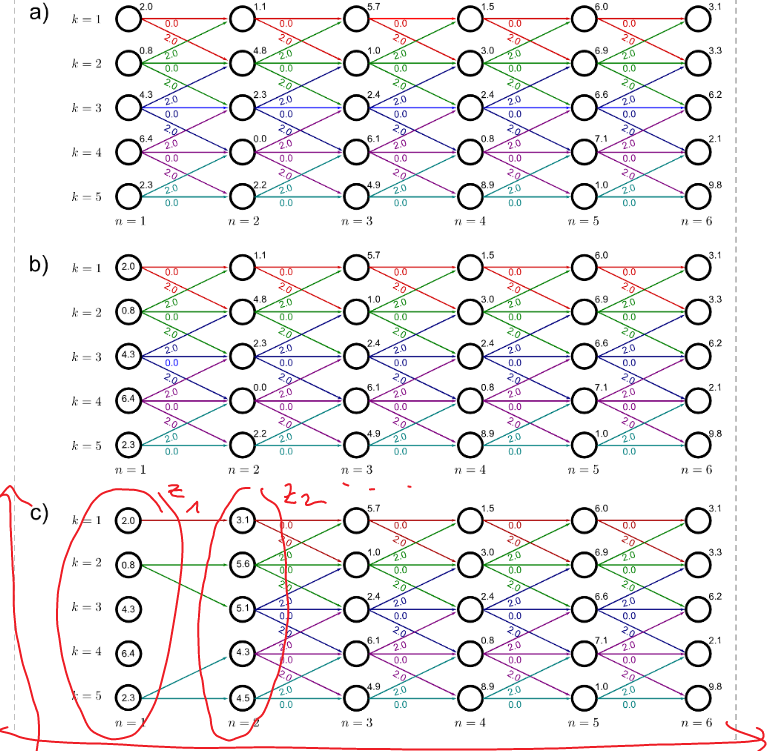
\includegraphics[width=0.6\textwidth]{Figures/state_vectors}
  \caption{State vectors}
\end{figure}

\section{Segmented least squares}

%%% Local Variables:
%%% mode: latex
%%% TeX-master: "../main"
%%% End:
